\section{Configuración de Arch Linux}
\subsection{Localización}
\begin{frame}

    {\color{blue}Editamos con {\ttfamily nano} {\color{red}\ttfamily /etc/locale.gen}}\\\vspace{3mm}

    \visible<1->{\begin{tcolorbox}[title=Aquí configuramos el idioma]
      \orden{nano /etc/locale.gen}
    \end{tcolorbox}}
    \visible<2->{\begin{tcolorbox}[title=Descomentamos la línea que contenga {\color{red}es\_ES.UTF-8 UTF-8}]
      \centering
      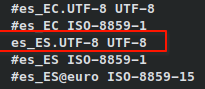
\includegraphics[width=30mm]{9 localizacion.png}\\
    \end{tcolorbox}}\pause
    
    \visible<3>{\begin{tcolorbox}[title=Y tras guardar:]
      \orden{locale-gen}
    \end{tcolorbox}}
    
\end{frame}

\begin{frame}
    \begin{tcolorbox}[title=Para establecer el idioma por defecto:]
	    \orden{echo 'LANG=es\_ES.UTF-8' > /etc/locale.conf}\\
    	\orden{echo 'KEYMAP=es' > /etc/vconsole.conf}
    \end{tcolorbox}
\end{frame}

